\documentclass[conference]{IEEEtran}

% *** CITATION PACKAGES ***
%
%\usepackage{cite}
% cite.sty was written by Donald Arseneau
% V1.6 and later of IEEEtran pre-defines the format of the cite.sty package
% \cite{} output to follow that of the IEEE. Loading the cite package will
% result in citation numbers being automatically sorted and properly
% "compressed/ranged". e.g., [1], [9], [2], [7], [5], [6] without using
% cite.sty will become [1], [2], [5]--[7], [9] using cite.sty. cite.sty's
% \cite will automatically add leading space, if needed. Use cite.sty's
% noadjust option (cite.sty V3.8 and later) if you want to turn this off
% such as if a citation ever needs to be enclosed in parenthesis.
% cite.sty is already installed on most LaTeX systems. Be sure and use
% version 5.0 (2009-03-20) and later if using hyperref.sty.
% The latest version can be obtained at:
% http://www.ctan.org/pkg/cite
% The documentation is contained in the cite.sty file itself.




% *** GRAPHICS RELATED PACKAGES ***
%
\ifCLASSINFOpdf
  \usepackage[pdftex]{graphicx}
  % declare the path(s) where your graphic files are
  % \graphicspath{{../pdf/}{../jpeg/}}
  % and their extensions so you won't have to specify these with
  % every instance of \includegraphics
  % \DeclareGraphicsExtensions{.pdf,.jpeg,.png}
\else
  % or other class option (dvipsone, dvipdf, if not using dvips). graphicx
  % will default to the driver specified in the system graphics.cfg if no
  % driver is specified.
  % \usepackage[dvips]{graphicx}
  % declare the path(s) where your graphic files are
  % \graphicspath{{../eps/}}
  % and their extensions so you won't have to specify these with
  % every instance of \includegraphics
  % \DeclareGraphicsExtensions{.eps}
\fi
% graphicx was written by David Carlisle and Sebastian Rahtz. It is
% required if you want graphics, photos, etc. graphicx.sty is already
% installed on most LaTeX systems. The latest version and documentatio4n
% can be obtained at: 
% http://www.ctan.org/pkg/graphicx
% Another good source of documentation is "Using Imported Graphics in
% LaTeX2e" by Keith Reckdahl which can be found at:
% http://www.ctan.org/pkg/epslatex
%
% latex, and pdflatex in dvi mode, support graphics in encapsulated
% postscript (.eps) format. pdflatex in pdf mode supports graphics
% in .pdf, .jpeg, .png and .mps (metapost) formats. Users should ensure
% that all non-photo figures use a vector format (.eps, .pdf, .mps) and
% not a bitmapped formats (.jpeg, .png). The IEEE frowns on bitmapped formats
% which can result in "jaggedy"/blurry rendering of lines and letters as
% well as large increases in file sizes.
%
% You can find documentation about the pdfTeX application at:
% http://www.tug.org/applications/pdftex


% *** MATH PACKAGES ***
%
%\usepackage{amsmath}
% A popular package from the American Mathematical Society that provides
% many useful and powerful commands for dealing with mathematics.
%
% Note that the amsmath package sets \interdisplaylinepenalty to 10000
% thus preventing page breaks from occurring within multiline equations. Use:
%\interdisplaylinepenalty=2500
% after loading amsmath to restore such page breaks as IEEEtran.cls normally
% does. amsmath.sty is already installed on most LaTeX systems. The latest
% version and documentation can be obtained at:
% http://www.ctan.org/pkg/amsmath


% *** SPECIALIZED LIST PACKAGES ***
%
%\usepackage{algorithmic}
% algorithmic.sty was written by Peter Williams and Rogerio Brito.
% This package provides an algorithmic environment fo describing algorithms.
% You can use the algorithmic environment in-text or within a figure
% environment to provide for a floating algorithm. Do NOT use the algorithm
% floating environment provided by algorithm.sty (by the same authors) or
% algorithm2e.sty (by Christophe Fiorio) as the IEEE does not use dedicated
% algorithm float types and packages that provide these will not provide
% correct IEEE style captions. The latest version and documentation of
% algorithmic.sty can be obtained at:
% http://www.ctan.org/pkg/algorithms
% Also of interest may be the (relatively newer and more customizable)
% algorithmicx.sty package by Szasz Janos:
% http://www.ctan.org/pkg/algorithmicx


% *** ALIGNMENT PACKAGES ***
%
%\usepackage{array}
% Frank Mittelbach's and David Carlisle's array.sty patches and improves
% the standard LaTeX2e array and tabular environments to provide better
% appearance and additional user controls. As the default LaTeX2e table
% generation code is lacking to the point of almost being broken with
% respect to the quality of the end results, all users are strongly
% advised to use an enhanced (at the very least that provided by array.sty)
% set of table tools. array.sty is already installed on most systems. The
% latest version and documentation can be obtained at:
% http://www.ctan.org/pkg/array


% IEEEtran contains the IEEEeqnarray family of commands that can be used to
% generate multiline equations as well as matrices, tables, etc., of high
% quality.


% *** SUBFIGURE PACKAGES ***
%\ifCLASSOPTIONcompsoc
%  \usepackage[caption=false,font=normalsize,labelfont=sf,textfont=sf]{subfig}
%\else
%  \usepackage[caption=false,font=footnotesize]{subfig}
%\fi
% subfig.sty, written by Steven Douglas Cochran, is the modern replacement
% for subfigure.sty, the latter of which is no longer maintained and is
% incompatible with some LaTeX packages including fixltx2e. However,
% subfig.sty requires and automatically loads Axel Sommerfeldt's caption.sty
% which will override IEEEtran.cls' handling of captions and this will result
% in non-IEEE style figure/table captions. To prevent this problem, be sure
% and invoke subfig.sty's "caption=false" package option (available since
% subfig.sty version 1.3, 2005/06/28) as this is will preserve IEEEtran.cls
% handling of captions.
% Note that the Computer Society format requires a larger sans serif font
% than the serif footnote size font used in traditional IEEE formatting
% and thus the need to invoke different subfig.sty package options depending
% on whether compsoc mode has been enabled.
%
% The latest version and documentation of subfig.sty can be obtained at:
% http://www.ctan.org/pkg/subfig




% *** FLOAT PACKAGES ***
%
%\usepackage{fixltx2e}
% fixltx2e, the successor to the earlier fix2col.sty, was written by
% Frank Mittelbach and David Carlisle. This package corrects a few problems
% in the LaTeX2e kernel, the most notable of which is that in current
% LaTeX2e releases, the ordering of single and double column floats is not
% guaranteed to be preserved. Thus, an unpatched LaTeX2e can allow a
% single column figure to be placed prior to an earlier double column
% figure.
% Be aware that LaTeX2e kernels dated 2015 and later have fixltx2e.sty's
% corrections already built into the system in which case a warning will
% be issued if an attempt is made to load fixltx2e.sty as it is no longer
% needed.
% The latest version and documentation can be found at:
% http://www.ctan.org/pkg/fixltx2e


%\usepackage{stfloats}
% stfloats.sty was written by Sigitas Tolusis. This package gives LaTeX2e
% the ability to do double column floats at the bottom of the page as well
% as the top. (e.g., "\begin{figure*}[!b]" is not normally possible in
% LaTeX2e). It also provides a command:
%\fnbelowfloat
% to enable the placement of footnotes below bottom floats (the standard
% LaTeX2e kernel puts them above bottom floats). This is an invasive package
% which rewrites many portions of the LaTeX2e float routines. It may not work
% with other packages that modify the LaTeX2e float routines. The latest
% version and documentation can be obtained at:
% http://www.ctan.org/pkg/stfloats
% Do not use the stfloats baselinefloat ability as the IEEE does not allow
% \baselineskip to stretch. Authors submitting work to the IEEE should note
% that the IEEE rarely uses double column equations and that authors should try
% to avoid such use. Do not be tempted to use the cuted.sty or midfloat.sty
% packages (also by Sigitas Tolusis) as the IEEE does not format its papers in
% such ways.
% Do not attempt to use stfloats with fixltx2e as they are incompatible.
% Instead, use Morten Hogholm'a dblfloatfix which combines the features
% of both fixltx2e and stfloats:
%
% \usepackage{dblfloatfix}
% The latest version can be found at:
% http://www.ctan.org/pkg/dblfloatfix




% *** PDF, URL AND HYPERLINK PACKAGES ***
%
%\usepackage{url}
% url.sty was written by Donald Arseneau. It provides better support for
% handling and breaking URLs. url.sty is already installed on most LaTeX
% systems. The latest version and documentation can be obtained at:
% http://www.ctan.org/pkg/url
% Basically, \url{my_url_here}.




% *** Do not adjust lengths that control margins, column widths, etc. ***
% *** Do not use packages that alter fonts (such as pslatex).         ***
% There should be no need to do such things with IEEEtran.cls V1.6 and later.
% (Unless specifically asked to do so by the journal or conference you plan
% to submit to, of course. )


% correct bad hyphenation here
\hyphenation{op-tical net-works semi-conduc-tor}


\begin{document}
%
% paper title
% Titles are generally capitalized except for words such as a, an, and, as,
% at, but, by, for, in, nor, of, on, or, the, to and up, which are usually
% not capitalized unless they are the first or last word of the title.
% Linebreaks \\ can be used within to get better formatting as desired.
% Do not put math or special symbols in the title.
\title{Stationary LIDAR Sensors for Indoor Quadcopter Localization }


% author names and affiliations
% use a multiple column layout for up to three different
% affiliations
\author{
\IEEEauthorblockN{Marcell Rausch, Gabor Feher}
\IEEEauthorblockA{Department of Telecommunication and Media Informatics\\
Budapest University of Technology and Economics, High Speed Network Laboratory, Budapest, Hungary}
}

% conference papers do not typically use \thanks and this command
% is locked out in conference mode. If really needed, such as for
% the acknowledgment of grants, issue a \IEEEoverridecommandlockouts
% after \documentclass

% for over three affiliations, or if they all won't fit within the width
% of the page, use this alternative format:
% 
%\author{\IEEEauthorblockN{Michael Shell\IEEEauthorrefmark{1},
%Homer Simpson\IEEEauthorrefmark{2},
%James Kirk\IEEEauthorrefmark{3}, 
%Montgomery Scott\IEEEauthorrefmark{3} and
%Eldon Tyrell\IEEEauthorrefmark{4}}
%\IEEEauthorblockA{\IEEEauthorrefmark{1}School of Electrical and Computer Engineering\\
%Georgia Institute of Technology,
%Atlanta, Georgia 30332--0250\\ Email: see http://www.michaelshell.org/contact.html}
%\IEEEauthorblockA{\IEEEauthorrefmark{2}Twentieth Century Fox, Springfield, USA\\
%Email: homer@thesimpsons.com}
%\IEEEauthorblockA{\IEEEauthorrefmark{3}Starfleet Academy, San Francisco, California 96678-2391\\
%Telephone: (800) 555--1212, Fax: (888) 555--1212}
%\IEEEauthorblockA{\IEEEauthorrefmark{4}Tyrell Inc., 123 Replicant Street, Los Angeles, California 90210--4321}}




% use for special paper notices
%\IEEEspecialpapernotice{(Invited Paper)}




% make the title area
\maketitle

% As a general rule, do not put math, special symbols or citations
% in the abstract
\begin{abstract}
Mobile robots need autonomous navigation, which cannot be fulfilled without proper localization. Today, there are various techniques for map creation and localization. However, most of them are not adequate for smaller devices, like quadcopters. In this paper, lightweight, small, and efficient stationary lidar sensors are proposed for localization. Through measurements and simulations, different sensor setups are investigated in the view of map creation quality and localization accuracy. Finally, the optimal sensor setup is presented with a minimal set of sensors, while the performance is still adequate.
\end{abstract}

% no keywords


% For peer review papers, you can put extra information on the cover
% page as needed:
% \ifCLASSOPTIONpeerreview
% \begin{center} \bfseries EDICS Category: 3-BBND \end{center}
% \fi
%
% For peerreview papers, this IEEEtran command inserts a page break and
% creates the second title. It will be ignored for other modes.
\IEEEpeerreviewmaketitle



\section{Introduction}
% no \IEEEPARstart
A prerequisite for future expansion of mobile robots is the ability to navigate autonomously and safely in 
their ever-changing environment without collisions. Simultaneous Localization And Mapping (SLAM) algorithms
discover the surroundings, create a map, and localize the robot in the map with the help of ranging or visual 
sensors. In an indoor scenario, this sensor is often the Light Detection and Ranging (LIDAR) sensor. 

Many papers can be found about SLAM and LIDAR sensors capable of building highly accurate maps of building-interiors or even outdoors \cite{engel2014lsd} \cite{mur2015orb} \cite{engel2015large}. However, they are using precise, long range rotating planner scanners,
which can be carried by a large industrial-grade hexacopter or octocopter only, and due to their weight, they are
not suitable for smaller quadcopters. Another frequent choice for drones is multiple cameras and image processing.
The issue here is the rather intense computation demand, which is hard to satisfy on a small quadcopter with 
limited power supply. 

In this paper, the evaluation of a SLAM system is introduced that uses stationary VL53L1X LIDAR sensors to scan
the drone's environment and uses Cartographer SLAM\cite{filipenko2018comparison}\cite{cartographerPaper} to construct maps. This solution might provide lightweight,
cheap, and computationally light alternative to currently used planar scanners. 

Each setup is evaluated based on data collected from Gazebo simulator \cite{GazeboWebsite}, and LIDAR sensors are simulated with 
parameters determined by measurements with VL53L1X sensors. On the collected data, multiple sensors layouts and 
settings were evaluated to find the optimal number of sensors and achieve a balance between accuracy and simplicity.


% An example of a floating figure using the graphicx package.
% Note that \label must occur AFTER (or within) \caption.
% For figures, \caption should occur after the \includegraphics.
% Note that IEEEtran v1.7 and later has special internal code that
% is designed to preserve the operation of \label within \caption
% even when the captionsoff option is in effect. However, because
% of issues like this, it may be the safest practice to put all your
% \label just after \caption rather than within \caption{}.
%
% Reminder: the "draftcls" or "draftclsnofoot", not "draft", class
% option should be used if it is desired that the figures are to be
% displayed while in draft mode.
%
%\begin{figure}[!t]
%\centering
%\includegraphics[width=2.5in]{myfigure}
% where an .eps filename suffix will be assumed under latex, 
% and a .pdf suffix will be assumed for pdflatex; or what has been declared
% via \DeclareGraphicsExtensions.
%\caption{Simulation results for the network.}
%\label{fig_sim}
%\end{figure}

% Note that the IEEE typically puts floats only at the top, even when this
% results in a large percentage of a column being occupied by floats.


% An example of a double column floating figure using two subfigures.
% (The subfig.sty package must be loaded for this to work.)
% The subfigure \label commands are set within each subfloat command,
% and the \label for the overall figure must come after \caption.
% \hfil is used as a separator to get equal spacing.
% Watch out that the combined width of all the subfigures on a 
% line do not exceed the text width or a line break will occur.
%
%\begin{figure*}[!t]
%\centering
%\subfloat[Case I]{\includegraphics[width=2.5in]{box}%
%\label{fig_first_case}}
%\hfil
%\subfloat[Case II]{\includegraphics[width=2.5in]{box}%
%\label{fig_second_case}}
%\caption{Simulation results for the network.}
%\label{fig_sim}
%\end{figure*}
%
% Note that often IEEE papers with subfigures do not employ subfigure
% captions (using the optional argument to \subfloat[]), but instead will
% reference/describe all of them (a), (b), etc., within the main caption.
% Be aware that for subfig.sty to generate the (a), (b), etc., subfigure
% labels, the optional argument to \subfloat must be present. If a
% subcaption is not desired, just leave its contents blank,
% e.g., \subfloat[].


% An example of a floating table. Note that, for IEEE style tables, the
% \caption command should come BEFORE the table and, given that table
% captions serve much like titles, are usually capitalized except for words
% such as a, an, and, as, at, but, by, for, in, nor, of, on, or, the, to
% and up, which are usually not capitalized unless they are the first or
% last word of the caption. Table text will default to \footnotesize as
% the IEEE normally uses this smaller font for tables.
% The \label must come after \caption as always.
%
%\begin{table}[!t]
%% increase table row spacing, adjust to taste
%\renewcommand{\arraystretch}{1.3}
% if using array.sty, it might be a good idea to tweak the value of
% \extrarowheight as needed to properly center the text within the cells
%\caption{An Example of a Table}
%\label{table_example}
%\centering
%% Some packages, such as MDW tools, offer better commands for making tables
%% than the plain LaTeX2e tabular which is used here.
%\begin{tabular}{|c||c|}
%\hline
%One & Two\\
%\hline
%Three & Four\\
%\hline
%\end{tabular}
%\end{table}


% Note that the IEEE does not put floats in the very first column
% - or typically anywhere on the first page for that matter. Also,
% in-text middle ("here") positioning is typically not used, but it
% is allowed and encouraged for Computer Society conferences (but
% not Computer Society journals). Most IEEE journals/conferences use
% top floats exclusively. 
% Note that, LaTeX2e, unlike IEEE journals/conferences, places
% footnotes above bottom floats. This can be corrected via the
% \fnbelowfloat command of the stfloats package.




\section{Ranging sensor-based SLAM}
Cameras are cheap, popular but they demand high processing capabilities. In contrast, ranging sensor-based 
approaches produce a lower amount of data and thus, they are less resource-intensive. Ultrasonic sensors have been used for distance measurements for many years, but they suffer from significant 
measurement noise. LIDAR sensors, on the other hand, use light to measure distance, offer more accurate 
measurements, typically lower form factor, higher resolution, and update rates. Planar scanners for 2D or 3D 
scanning typically use a rotating LIDAR sensor that makes evenly distributed measurements.

Stationary LIDAR sensor-based modules can be found for collision avoidance. TeraBee offers an off-the-shelf 
system with 8 selectable LIDAR sensors. The company offers long-range and fast-ranging versions, that can range
up to 60m or 600Hz.

Bitcraze has developed a Multi-ranger deck for their mini drone that weighs only 27g. This deck carries 5 VL53L1X
lidar sensors, 4 horizontally, and 1 vertically. The company website has a SLAM demo but provided no information
of the SLAM algorithm in use. 

\section{The VL53L1X LIDAR sensor}

VL53L1X is described as a long-distance ranging Time-of-Flight sensor by STMicroelectronics \cite{VL53L1XDatasheet}. 
The size of the module is 4.9x2.5x1.56mm, it emits 940nm invisible laser and uses a single-photon avalanche diode 
(SPAD) receiving array with a field-of-view(FOV) of 27 degrees. The module runs all the digital signal processing on a 
built-in low power microcontroller that frees up the host processor from these tasks. According to the datasheet, 
the sensor is capable of 50Hz ranging frequency and up to 400cm distance measurements. The size of the laser 
receiving array can be programmatically changed by setting the region-of-interest(ROI) size. 



The most relevant settings of the sensor are the timing budget, distance preset, and the resolution.
The timing budget sets the maximum time available for the sensor to complete ranging. It can be adjusted 
between 18.5ms to 1s. Distance preset sets 
the expected range distance, and by moving the ROI across the whole field-of-view, higher scan resolution 
can be achieved. Using this method, the resolution can be extended to 4x4 without overlapping segments.

To simulate the VL53L1X sensor accurately, a series of measurements were conducted on distances from 0.5m to 4m
in 0.5m steps with selected sensor settings. On each distance, the average measured distance, standard deviation,
sampling rate, and typical range status were measured with the selected settings. Measurements were done with 
sensor resolutions 1x1, 2x2, 3x3, 4x4, and all distance presets: short, medium, long. It is unnecessary to test
the sensor with all possible timing budget values, so 4 values have been selected.
18.5 ms provides the highest sampling rate of 50Hz, but can only be used with short-distance preset. 33ms is the 
lowest timing that can be used with long-distance preset. Based on the datasheet, 140ms is the lowest budget that
can provide ranges up to 400cm, and lastly, 200ms is expected to provide less noisy measurements.
The last three values are also used in the VL53L1X datasheet\cite{VL53L1XDatasheet} to demonstrate ranging 
accuracy. 
\begin{figure}[!t]
\centering
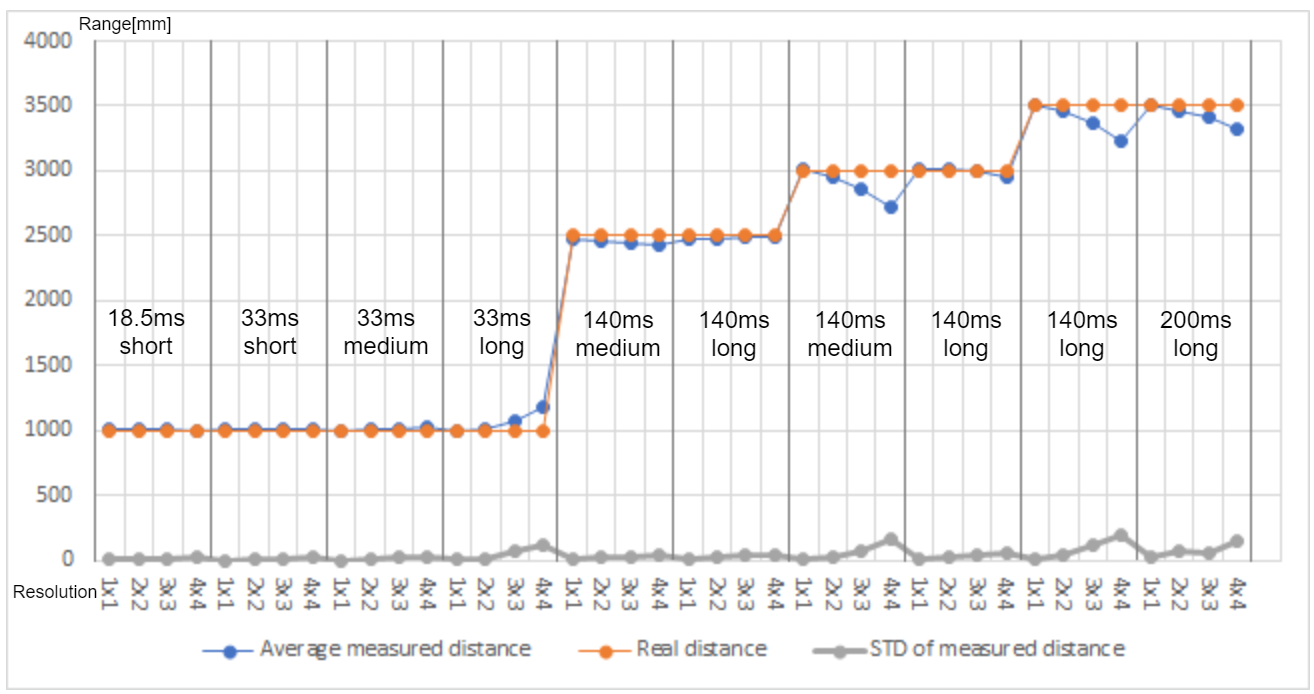
\includegraphics[width=0.5\textwidth]{vl53l1x_measurements_opmodes.png}
% where an .eps filename suffix will be assumed under latex, 
% and a .pdf suffix will be assumed for pdflatex; or what has been declared
% via \DeclareGraphicsExtensions.
\caption{VL53L1X measurements.}
\label{fig_measurements}
\end{figure}

Based on the completed measurements, it can be seen that sampling time is independent of the distance preset 
and is directly proportional to the resolution and the timing budget. In each tested 
scenario, the most accurate measurements were always with resolution 1x1. By increasing the resolution, therefore
lowering the receiver SPAD array size, the measured distance starts to deviate from the real distance, and 
standard deviation increases. This can be seen at 2.5m distance with medium preset in figure \ref{fig_measurements}. Long-distance preset, 
however produces more accurate measurements even on 3m, so it is preferred over medium preset. Measurements 
with long-distance preset and 140ms timing budget follow the real distances even on 3 meters but start to 
deviate at 3.5 meters with 2x2-resolution and above. Raising the timing budget to 200ms reduces the error 
and standard deviation, but the error is still significant.

18.5ms timing budget with short distance preset can produce the fastest ranging measurements up to 1.6m according
to the datasheet. The short preset also has the best ambient light immunity, a favorable quality. Surprisingly,
in the tests, the sensor with these settings was able to measure up to 2m with only 7mm standard deviation only. 
Above 2m no ranges were successful. Compared to other presets, the sampling time for each resolution decreased
significantly. In the case of 4x4-resolution, the sampling time has decreased from 390ms to 265ms, and the 
maximum distance decreased from 2.5m to about 1m. The increase in the update rate might be beneficial for 
the SLAM algorithm. 

\section{2D SLAM evaluation}

To be able to compare the performance of the SLAM algorithm with each sensor setup, the same dataset 
is used. The collected data contains LIDAR measurements of the surroundings of the vehicle in 3D. In the Gazebo simulator, 
LIDAR scanners are placed on the top and bottom of the quadcopter to evenly scan the top- and bottom 
hemispheres. The drone was flown around inside a simulated building, that was designed to have rooms that only 
have distances under the maximum distance of the ranging sensor and bigger rooms so that some ranges  
can be saturated. The building contains no furniture but has doors and windows. All sensor and control messages are recorded. The LIDAR measurements update at 30Hz, while IMU is published at 50Hz.

The recorded data is filtered to simulate the VL53L1X sensors in a specific layout, all with the same settings. 
Sensor parameters are determined using the measurements with the actual sensor. These simulation parameters are
the sampling rate and maximum distance. 

The filtered data is played back for Cartographer SLAM, that is tuned to have the best possible performance
with the current setup. Tuning requires a good understanding of the parameters, and the procedure is unique for
each setup. At first, the algorithm is tuned to build stable and consistent submaps, then for global SLAM and
loop closures.

To have an absolute measure besides visual inspection, the RMS error is calculated of the SLAM trajectory of 
each setup. The ground-truth trajectory is provided by Gazebo.
 
The LIDAR parameters are introduced incrementally, starting from unfiltered range data, that is expected to 
result in the best possible map and trajectory using this dataset. Sensor resolution, sampling rate and 
maximum distance limit are introduced after each other to see their effects individually. 13 sensors are used
in even layout on the horizontal plane for the evaluation process. Finally, the number of sensors is reduced
until the SLAM algorithm is still capable of consistent and reliable mapping.

\subsection{Effects of LIDAR resolution}

First, unfiltered data ranges with maximum rate and distance were used, without additional noise.
Even without global SLAM, a decent quality map could be built. The extracted trajectory closely followed 
the ground-truth trajectory. The RMS error on the x- was 6.3cm and a bit less 6.5cm on the y-axis, resulting 
in a cumulated 9.05cm RMS error. The lowered resolution introduces an artifact, that is referred to as transition
point. These points appear when the ROI is partly covered by a close object and the rest is by a far object, so 
the reported distance is in between the two obstacles. For example, this causes corners to be curved on lower 
resolutions.

4x4 and 3x3 resolutions provide a high number of points per scan, which makes scan matching more effective. 
Mapping accuracy and map building reliability are decent for both cases, but 3x3 produced slightly lower RMS error.
This might be because of more efficient tuning. 

2x2 and 1x1 resolutions have significantly fewer points per scan that makes tuning of Cartographer significantly 
harder. 1x1 proved to be unreliable, and the algorithm was unable to match scans to build submaps. 
The map built using 2x2 resolution resulted in curved corners and blurry edges. Lowered grid resolution 
resulted in higher accuracy and stability.

\begin{table}[!t]
% increase table row spacing, adjust to taste
\renewcommand{\arraystretch}{1.3}
% if using array.sty, it might be a good idea to tweak the value of
% \extrarowheight as needed to properly center the text within the cells
\caption{RMS error of different resolutions}
\label{table_resolution}
\centering
% Some packages, such as MDW tools, offer better commands for making tables
% than the plain LaTeX2e tabular which is used here.
\begin{tabular}{|c||c|c|c|c|}
\hline
  & 4x4 & 3x3 & 2x2 & 1x1\\
\hline
\hline
x [cm] & 8.12 & 4.04 & 7.95 & -\\
\hline
y [cm]& 10.48 & 7.3& 14.17& -\\
\hline
sum [cm]& 13.26 & 8.34 & 16.25& -\\
\hline
\end{tabular}
\end{table}




% \subsubsection{4x4-resolution}

% In this scenario, the filter selected 4 times 52 points around the quadcopter in 4 rows. This scenario has 
% the least amount of artifacts compared to the lower resolution. The estimated trajectory followed accurately the 
% ground-truth trajectory. There were no constant offsets on either ax. The RMS error was 8.12cm on the x- and 
% 10.48cm on the y-axis, resulting in a cumulated error of 13.26cm. 

% \subsubsection{3x3-resolution}

% As the resolution is lowered to 3x3, the field of view of each region of interest had broadened. This caused 
% the transition points to be more significant, that has an impact on the performance of the system. 
% Tuning on the SLAM algorithm helped to produce a decent quality map and the global SLAM was able to compensate 
% drifting submaps. Although the mapping quality was reduced due to the the reduced sensor resolution, the 
% localization accuracy had increased. The cumulated RMS error for this setup was 8.34cm. The RMS error on 
% the x- was 4.04cm and on the y-axis it was 7.3cm. The accuracy of this setup is the result of the better 
% SLAM parameter tuning. 

% \subsubsection{2x2 and 1x1 resolutions}

% Compared to the 3x3-resolution, these scenario contains relevantly fewer points, which makes scan matching 
% significantly less efficient. Tuning of this setup was noticeably harder and the quality of the produced map 
% was highly decreased. The grid resolution of the map should be reduced to low resolution. While the configuration
%  with a high-resolution grid map was able to follow the ground-truth trajectory in small rooms and the narrow 
%  corridor, it lost track in the big and spacious room, when the ranges were far apart. 

% In the case of the 2x2-resolution, the high-resolution trajectory was at some points as far as 1.4m from the
% ground-truth pose, but the cumulated RMS error was only 43.4cm. This shows that a seemingly small difference in 
% RMS error can mean an error of more than a meter at a part of the trajectory. The low-resolution trajectory in
% comparison has a cumulated RMS error of 22.13cm. 7.95cm error on the x- and 14.17cm on the y-axis. The 
% 1x1-resolution scenario did not produce any usable map or localization. 

% These scenarios were unusable for the SLAM, so they were not tested further.  




\subsection{Effects of sampling rate}

For the 4x4-resolution 400ms sampling time was chosen, based on the real sensor measurements. The dropped 
sampling rate 
from 30Hz to 2.5Hz was significant and made the tuning much harder. Two different grid resolutions were tested 
as well. The quality of the map was decent in both cases, and no major flaws were visible. The global SLAM had to 
compensate rotation drifts, that occurred when the drone quickly turned around in the big room, where some 
ranges became saturated. Low grid resolution produced a smoother path, while on the high-resolution grid, there 
were jumps and sharper turns. 

The cumulated RMS error on a high grid resolution was 16.49cm. On low grid resolution, it was higher: 18.95cm. 
Higher grid-resolution results in greater accuracy in position estimates, but its stability is lower in comparison
to a lower resolution. 

As for the 3x3-resolution, the same sensor settings were chosen, but this setup has a better sampling time of 
220ms compared to the previous 400ms. This results in an 80\% increase in update rate to 4.5Hz, which also 
means almost twice more often pose updates. Lowering the grid resolution was necessary here as well. The map 
quality was adequate, and global SLAM almost has not done any corrections. The cumulated RMS error was 10.4cm, 
6.4cm on the x-axis, and 8.2 on the y-axis. Because of stability and accuracy, 3x3-resolution seems like a 
better resolution for Cartographer SLAM. 

\subsection{Effects of maximum distance}

The VL53L1X sensor measurements showed that each setup works accurately until 2.5m and each has about 25cm 
drift at a distance of 3m, so 2.75m as the maximum distance was chosen for the tests. The lowered maximum 
distance had a positive effect that the number of transition points has been reduced because on the shorter 
distance, the field of view could not open as wide as it could before. The downside of the limited range is 
that the algorithm loses track in the open spaces. This caused more flaws, and a small tilt can be observed
in the map.  
The trajectory using sensors with 3x3-resolution has a significant offset on the y-axis, which was picked up 
due to the reduced reference points. Similar scans were pulled together, resulting for example in a shortened
corridor. 
The trajectory using 4x4-resolution sensors has a smaller offset. It seems like with more 
points per scan, the SLAM algorithm was able to pick up small details and better track the movement of the 
drone even on a mostly even corridor. On the other hand, it failed in a big room with significantly greater 
distances than 2.75m.

The cumulated RMS error for 3x3-resolution is 38.16cm and 35.12cm for 4x4. This also showed that a mostly
constant offset with otherwise correct shape results in a smaller error, than the pose estimation that 
follows ground-truth closely but failed in shape at a relatively small area. 

\subsection{Reduced set of evenly distributed LIDAR sensors}

In this test, the goal was to find the minimum number of LIDAR sensors, with which the SLAM algorithm still 
works reliably and can produce a coherent map. The sensors were set to 4x4 and 3x3-resolution, 400ms update 
rate, and 2.75m as maximum distance. The tuning of the algorithm proved to be significantly harder this time. 
8 sensors proved to be the lowest, using 7 already caused the submaps to fall apart. The RMS cumulated error 
was 34.1cm for 4x4, while mapping has failed using 3x3-resolution. The map and trajectory built using 8 sensors
can be seen in figure \ref{fig_8_sensors}.

\begin{figure}[!t]
  \centering
  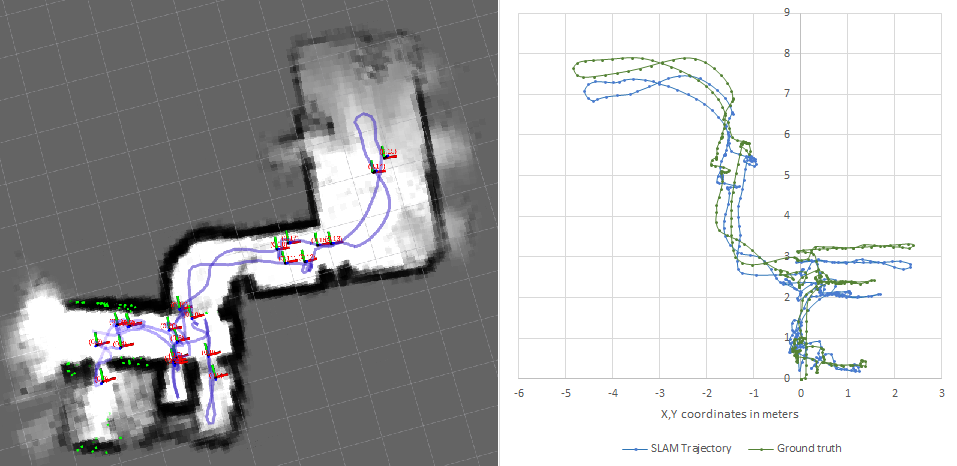
\includegraphics[width=0.5\textwidth]{08_map_8sensor_4x4.png}
  % where an .eps filename suffix will be assumed under latex, 
  % and a .pdf suffix will be assumed for pdflatex; or what has been declared
  % via \DeclareGraphicsExtensions.
  \caption{Map trajectory using 8 LIDAR sensors}
  \label{fig_8_sensors}
  \end{figure}

\section{Conclusion}
Indoor quadcopters require lightweight localization systems for navigation. An option for this task could be the application of stationary LIDAR sensors. The performance evaluation presented in this paper has shown that it is possible indeed to perform adequate localization using such sensors. In addition to the measurement and simulation analysis of different sensor setups, an optimal sensor configuration was presented. In this setup, there should be 8 stationary LIDAR sensors, as fewer sensors make the localization to fail.


% conference papers do not normally have an appendix


% use section* for acknowledgment
\section*{Acknowledgment}
This work has been supported by the Ericsson - BME 5G
joint research and cooperation project, partly funded by the
National Research, Development and Innovation Office,
Hungary, project number 2018-1.3.1-VKE-2018-00005.


% trigger a \newpage just before the given reference
% number - used to balance the columns on the last page
% adjust value as needed - may need to be readjusted if
% the document is modified later
%\IEEEtriggeratref{8}
% The "triggered" command can be changed if desired:
%\IEEEtriggercmd{\enlargethispage{-5in}}

% references section

% can use a bibliography generated by BibTeX as a .bbl file
% BibTeX documentation can be easily obtained at:
% http://mirror.ctan.org/biblio/bibtex/contrib/doc/
% The IEEEtran BibTeX style support page is at:
% http://www.michaelshell.org/tex/ieeetran/bibtex/
\bibliography{biblio}
\bibliographystyle{IEEEtran}
% argument is your BibTeX string definitions and bibliography database(s)
%
% <OR> manually copy in the resultant .bbl file
% set second argument of \begin to the number of references
% (used to reserve space for the reference number labels box)
% \begin{thebibliography}{1}
% \end{thebibliography}


% that's all folks
\end{document}


